\documentclass[12pt]{article}
\usepackage[colorinlistoftodos]{todonotes}
\usepackage{amsmath}
\usepackage{amssymb}
\usepackage{bm}
\usepackage{enumerate}
\usepackage{fancyvrb}
\usepackage[top=1in, bottom=1in, left=1in, right=1in]{geometry}
\usepackage{hyperref}
\usepackage{placeins}
\usepackage{tikz}
\usepackage{tikzsymbols}
\usepackage{todonotes}
\usepackage{bbm}
\usepackage{color}
\usepackage{mathrsfs}
\usepackage{enumitem}
\usepackage{soul} % for HL
\usepackage{color} % for HL
\usepackage{listings}
\usepackage{xcolor}
\usepackage{graphicx}
\graphicspath{{./images/}}

\definecolor{codegreen}{rgb}{0,0.6,0}
\definecolor{codegray}{rgb}{0.5,0.5,0.5}
\definecolor{codepurple}{rgb}{0.58,0,0.82}
\definecolor{backcolour}{rgb}{0.95,0.95,0.92}
\newcommand\iid{i.i.d.}
\lstdefinestyle{mystyle}{
    backgroundcolor=\color{backcolour},   
    commentstyle=\color{codegreen},
    keywordstyle=\color{magenta},
    numberstyle=\tiny\color{codegray},
    stringstyle=\color{codepurple},
    basicstyle=\ttfamily\footnotesize,
    breakatwhitespace=false,         
    breaklines=true,                 
    captionpos=b,                    
    keepspaces=true,                 
    numbers=left,                    
    numbersep=5pt,                  
    showspaces=false,                
    showstringspaces=false,
    showtabs=false,                  
    tabsize=2
}

\lstset{style=mystyle}

% \renewcommand{\theenumi}{\roman{enumi}}
\newcommand{\rmn}[1]{{\textcolor{blue}{\bf [{\sc rmn:} #1]}}}
\DeclareMathOperator*{\argmax}{arg\,max}

\usetikzlibrary{positioning,calc}
%%%%%%%%%
\usepackage[most]{tcolorbox}
\newtcolorbox[]{solution}[1][]{%
    breakable,
    enhanced,
    colback=white,
    title=Solution,
    #1
}

\newtcolorbox[]{fillme}[1][]{%
    breakable,
    enhanced,
    colback=white,
    title=Fill me in,
    #1
}

\newcommand*{\E}{\mathbb{E}}
\newcommand*{\prob}{\mathbb{P}}
\newcommand*{\F}{\mathcal{F}}
\newtheorem{theorem}{Theorem}
\newtheorem{observation}{Observation}
\newtheorem{corollary}[theorem]{Corollary}
\newtheorem{definition}[theorem]{Definition}
\newtheorem{lemma}[theorem]{Lemma}
\newtheorem{proposition}[theorem]{Proposition}

%%%%%%%%%%
\title{ECE433/COS435 Introduction to RL\\
  Assignment 0: Review of Topics\\
  Spring 2025\\
}

\date{Due February 3, 2025}
\author{\begin{fillme}[width=0.3\textwidth]
Yuzhou Zhao
\end{fillme}} % Fill in your name!

\begin{document}

\maketitle
\noindent

\begin{itemize}
    \item This homework has a \texttt{hw0.ipynb} file for the programming sections. Please also download the file. All answers should be provided in this PDF file instead of the \texttt{hw0.ipynb} file and you will \textbf{only submit this PDF}. The solution code should be pasted into the corresponding answer blocks.
    \item This assignment will be graded out of 0 points, which means it will not be included in your final grade.
    \item For coding questions in this assignment, you can compile the code on your own laptop or \href{https://colab.research.google.com/}{Google Colab}. We will be providing all students with access to Adroit for future assignments. We would recommend to use Colab as the questions and package dependencies have been verified on it.
\end{itemize}

\newpage
\section*{Collaborators}
\begin{fillme}
You should work alone for this assignment.
\end{fillme}

\section*{Instructions}

You should work alone for this assignment. Writeups should be typeset in Latex and submitted as PDF. You can work with whatever tool you like for the code, but \textbf{please submit the asked-for snippet and answer in the solutions box as part of your writeup. We will only be grading your writeup.} Make sure to still also attach your notebook/code with your submission.

\section*{Introduction}
This Homework is meant to be a review of standard topics on machine learning, linear algebra, and probability, with a heavy emphasis on topics that will reappear in later stages of this course. 
\\\\
You will also work with PyTorch and Python to build your models, so we want to make sure you are familiar with the specific packages (e.g. \texttt{torch.distributions}) that you will be using throughout the course.
\newpage

% ----------------- QUESTION 1 ----------------- %

\section*{Question 1. Probability (0 points)}
In a reinforcement learning setting, we are often interested in settings where an agent interacts with a game environment. We often want to learn the agent's policy $\pi$, or its ``rule" for making actions. In this problem, you will derive properties of different ``rules" over a simple game, and it helps you to understand the policy from a statistical perspective.
\\\\
Suppose we are playing a really simple game with $10$ unique boxes, each with their own distinct label from $1,...,10$. One of these boxes contains a golden coin that awards the player with a reward of $5$, one contains a silver coin that awards the player with a reward of $1$, and the rest contain nothing and award the player with a reward of $0$ if selected. The player must open a single box, and based on the outcome, their final score is the reward corresponding to the box that they selected. More formally, the player has a policy $\pi$ and uses it to select an action $a \sim \pi$ corresponding to the box the player picked (e.g. $a=1$ means the player picked box $1$). The player is then given a reward $r(a)$ based on their action.

\subsection*{Question 1.a (0 points)}

Suppose our \textbf{agent's policy} is to randomly select one of the labelled boxes,\href{https://en.wikipedia.org/wiki/Discrete_uniform_distribution}{ each with equal probability}. In other words, $\pi = \mathcal{U}\{1,\dots, 10\}$, and the agent selects a box $a \sim \pi$. Conditioned on the fact the the gold coin is in the box labelled $5$ and the silver coin is in box labeled $1$, what is the expected reward?

\begin{solution}
Know that:
\begin{equation}
    r(a) = \begin{cases}
5, & a = 5, \\
1, & a = 1, \\
0, & \text{otherwise }.
\end{cases}
\end{equation}
Thus the expected reward is: 
\begin{align}
    \mathbb{E}[r(a)] = & \sum_{a=1}^{10}P(a)r(a) \\
    = & \frac{1}{10}\cdot 5 +\frac{1}{10}\cdot 1 \\
    = & 0.6
\end{align} 
\end{solution}

\subsection*{Question 1.b (0 points)}
Given the same assumptions as (1.a), what is the policy of the agent that maximizes the expected reward?
\begin{solution}
The policy that maximized the expected reward would be 
\begin{equation}
    \pi^* = \delta(a=5) = \begin{cases}
1, & a = 5, \\
0, & \text{otherwise }.
\end{cases}
\end{equation}
And the maximized reward is $\mathbb{E}[r(a\sim \pi^*)] = 5$

\end{solution}

\subsection*{Question 1.c (0 points)}
What is the entropy of the policy in (1.a) and the entropy of the policy in (1.b)? 

\begin{solution}
The entropy of the first policy $\pi$:
\begin{equation}
    H(\pi) = -\sum_{a=1}^{10}P(a)\log P(a) = -\sum_{a=1}^{10}\frac{1}{10}\log \frac{1}{10} \cong 3.32
\end{equation}
The entropy of the second policy $\pi^*$:
\begin{equation}
    H(\pi^*) = -\sum_{a=1}^{10}P(a)\log P(a) = -\log 1 = 0 .
\end{equation}
Which means that the second policy has no uncertainty at all.
\end{solution}

\subsection*{Question 1.d \textbf{Coding} (0 points)}
Suppose instead of boxes, we now deal with a \textit{continuous} set of possible decisions. In this scenario, our agent can choose any number $a \in \mathbb{R}$, and the reward given to the player is defined by
$$
    \mathcal{R}(x) = \max \biggr \{ 0, 1 - |x - 1| \biggr\}
$$
In this problem, you will use this reward function to compute the expected return of a policy (to be 
defined). The key idea is that an expectation can be approximated through sampling (\href{https://princeton-introml.github.io/files/ch15.pdf}{recall Monte Carlo sampling from COS324}). In this problem, you will familiarize yourself with the \href{https://pytorch.org/docs/stable/distributions.html}{\texttt{torch.distributions}} library.
\\\\
See the colab notebook (1.d) (in \texttt{hw0.ipynb} file) for more details. Fill 
out the indicated code segments below after solving 
the problem.

\begin{solution}
Expected reward is \textbf{0.58 to the nearest hundredth, 0.6 to the nearest tenth as specified in the ipynb file}. 
\\\\
\textbf{Fill in your code here:}
\begin{lstlisting}[language=Python]
### Your code here.
g_x = Normal(0.6, 0.3)
x = g_x.sample((100000,))
r = reward(x)
print("Expected reward:", r.mean())
\end{lstlisting}
\end{solution}

\newpage
\subsection*{Question 1.e \textbf{Coding} (0 points)}
Plot the reward distribution under this policy using \texttt{matplotlib.pyplot.hist()} or some other histogram plotting library. Make sure to label your axes for this problem (x-axis is reward, y-axis is probability density). See colab notebook (1.e) (in \texttt{hw0.ipynb} file) for more details.
\\\\
\textit{\textbf{Hint.} When using \texttt{matplotlib.pyplot.hist()}, please output a \texttt{.png} file and fill it also in below answer block! (check the documentation.)}

\begin{solution}
\begin{lstlisting}[language=Python]
### Your code here.
plt.hist(r, bins=100, density=True)
plt.xlabel('r')
plt.ylabel('p(r)')
plt.savefig('q_1e.png')
\end{lstlisting}

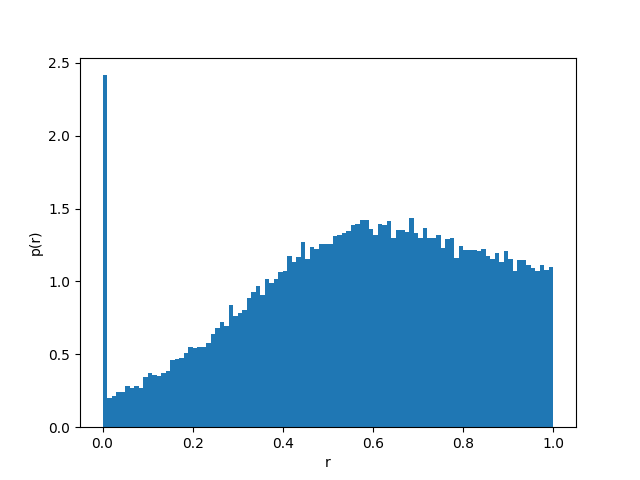
\includegraphics[width = \textwidth]{hw/HW0/q_1e.png}

\end{solution}
\newpage

% ----------------- QUESTION 2 ----------------- %
\section*{Question 2. MLE (0 points)}
The purpose of this question is to review Maximum Likelihood Estimation (MLE), which appears in many machine learning settings. You may have seen or solved a few questions on computing the Maximum Likelihood Estimator for a set of datapoints, in which case this problem will be a review.
\\\\
A random variable $X$ has a Normal distribution with parameters $\mu,\sigma^2$ if its probability distribution is uniquely defined as
$$ f_X(x) = \frac{1}{\sqrt{2\pi \sigma^2}} \exp \left( - \frac{(x - \mu)^2}{2\sigma^2} \right).  $$

\subsection*{Question 2.a (0 points)} 
Let $\theta = \sigma^2$. For a set of datapoints $X_1,...,X_n$ sampled \iid~from a Normal distribution with unknown parameters $\mu$ and $\theta$, find the log-likelihood function $L(\mu, \theta; X_1,...,X_n)$. You answer should be in terms of $n$, $X_1,...,X_n$, $\mu$, and $\theta$.

\begin{solution}
\begin{align}
    L(\mu, \theta; X_1,...,X_n) = & \ln \left(\prod_{i=1}^{n}f_X(\mu, \theta; X_i)\right) \\
    = & \sum_{i=1}^{n}\ln \left( \frac{1}{\sqrt{2\pi \theta}} \exp \left( - \frac{(X_i - \mu)^2}{2\theta} \right) \right) \\
    = & \sum_{i=1}^{n}\ln \left( \frac{1}{\sqrt{2\pi \theta}} \right) - \frac{(X_i - \mu)^2}{2\theta} \\
    = & -\frac{n}{2} \ln \left( 2 \pi \theta \right) - \sum_{i=1}^{n} \frac{(X_i - \mu)^2}{2\theta}
\end{align}

\end{solution}
\subsection*{Question 2.b (0 points)} 
Using your answer in (2.a), solve for the MLE of $\mu$ and $\theta$. Solutions should also show that the critical points are maximums, e.g., compute derivatives around the critical point and number of critical points argument.
\begin{solution}
$\frac{\partial L}{\partial \mu}=\sum_{i=1}^{n} \frac{X_i - \mu}{\theta}$

$\frac{\partial L}{\partial \theta}= -\frac{n}{2\theta} + \sum_{i=1}^{n} \frac{(X_i - \mu)^2}{2\theta^2}$
\end{solution}
\newpage

% ----------------- QUESTION 3 ----------------- %
\section*{Question 3. Coding (0 points) }
The objective of this question is to familiarize you with the basic mechanics of PyTorch and Python. The question descriptions and code templates are provided in the provided \texttt{hw0.ipynb}, please see \textbf{Question 3} in the \texttt{hw0.ipynb} notebook. You will program gradient descent and building a basic neural network model in this question.

\subsection*{Question 3.a (0 points) } 
For this problem and (3.b), see the provided \texttt{hw0.ipynb} notebook for all the questions, and fill out the indicated code segments below after solving 
each problem.

\begin{solution}
\begin{lstlisting}[language=Python]
# Import the dataset
rng = np.random.RandomState(189289213)
X = 10 * rng.rand(1000, 10) # feature matrix
y = np.dot(X, [1,2,3,4,5,6,7,8,9,10]) + np.random.normal(0, 0.01) # target vector

def init_weights (in_1:int, in_2:int) -> np.ndarray:
  return np.random.rand(in_1,in_2)

weights = init_weights(X.shape[1], 1)

# Helper functions to get you started. Feel free to use or not use them.
def gradient_descent(X, y, weights: np.ndarray, eta: float, iterations: int):
  for i in range(iterations):
    ### Your code here.
    N = X.shape[0]
    loss = 1 / (2*N) * (X @ weights - y[:, None]).T @ (X @ weights - y[:, None])
    grad = X / N * (X @ weights - y[:, None])
    weights -= eta * grad.sum(0)[:, None]
    if i % 100 ==0: print("loss: ", loss) 

gradient_descent(X, y, weights, eta=0.001, iterations=500)

print("Solved weights:", weights)
'''
loss:  [[34301.87999235]]
loss:  [[62.24029559]]
loss:  [[12.82772996]]
loss:  [[2.69173858]]
loss:  [[0.57378897]]
Solved weights: [[1.10131518]
 [2.06274845]
 [3.03431916]
 [4.03897822]
 [5.00152001]
 [5.99416033]
 [6.97466198]
 [7.93863466]
 [8.90699561]
 [9.94703617]]
'''
\end{lstlisting}
\end{solution}

\subsection*{Question 3.b (0 points) } 
Rewrite your solution to (3.a) using the torch library. Your solution must use \texttt{loss.backward()} and \texttt{weight.grad}.

\begin{solution}
\begin{lstlisting}[language=Python]
X_t = torch.from_numpy(X).float()
y_t = torch.from_numpy(y).float()

weights = torch.randn((X.shape[1], 1), requires_grad=True)

def gradient_descent_torch(X, y, weights: torch.tensor, eta: float, iterations: int) -> None:
  for i in range(iterations):
    # Your code here
    N = X.shape[0]
    loss = 1 / (2*N) * (X @ weights - y.unsqueeze(-1)).T @ (X @ weights - y.unsqueeze(-1))
    loss.backward()
    with torch.no_grad(): 
      weights.sub_(eta * weights.grad)
    weights.grad.zero_()
    if i % 100 ==0: print("loss: ", loss) 

gradient_descent_torch(X_t, y_t, weights, 0.001, 500)
print(weights)
'''
loss:  tensor([[36692.4453]], grad_fn=<MmBackward0>)
loss:  tensor([[80.2165]], grad_fn=<MmBackward0>)
loss:  tensor([[16.3264]], grad_fn=<MmBackward0>)
loss:  tensor([[3.3814]], grad_fn=<MmBackward0>)
loss:  tensor([[0.7109]], grad_fn=<MmBackward0>)
tensor([[1.0877],
        [2.1002],
        [3.0348],
        [4.0425],
        [4.9941],
        [5.9777],
        [6.9692],
        [7.9612],
        [8.8860],
        [9.9462]], requires_grad=True)
'''
\end{lstlisting}
\end{solution}

\section*{Question 4. Feedback (0 points)}
We value your feedback and would love to hear your thoughts on the course. In one or two sentences, what are your goals for this course? Do you have any question about the material covered so far? Or do you have any suggestion on the course structure and contents to be covered? Your input is greatly appreciated!

% We value your feedback and would love to hear your thoughts on the course. Please share your feedbacks, including what you expect to change in course structure or logistics, areas for improvement, and any specific expectations or topics you would like us to cover in the future. Additionally, we welcome any suggestions on how we can enhance the learning experience to better meet your needs. Your input is greatly appreciated!
\begin{solution}
Upload Percept notes please.
\end{solution}

% \end{solution}
\newpage

\end{document}